\documentclass[10pt]{article}
\usepackage[utf8]{inputenc}
\usepackage[T1]{fontenc}
\usepackage{amsmath}
\usepackage{amsfonts}
\usepackage{amssymb}
\usepackage[version=4]{mhchem}
\usepackage{stmaryrd}
\usepackage{graphicx}
\usepackage[export]{adjustbox}
\graphicspath{ {./images/} }
\usepackage{caption}

\begin{document}
\captionsetup{singlelinecheck=false}
\section*{CHEMISTRY}
\section*{SECTION-A}
\begin{enumerate}
  \setcounter{enumi}{30}
  \item In the following halogenated organic compounds the one with maximum number of chlorine atoms in its structure is :\\
(1) Chloral\\
(2) Gammaxene\\
(3) Chloropicrin\\
(4)Freon -12
\end{enumerate}

Official Ans. by NTA (2)\\
Allen Ans. (2)

Sol. (1) Chloral\\
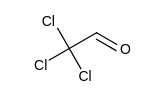
\includegraphics{smile-fd6c31d06dd11b1a80131ad053d63f193904915d}\\
(2) Gammaxene\\
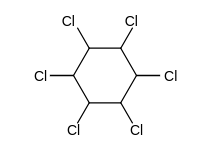
\includegraphics{smile-1ef58fbaca51777a39836c00da8477a8c52a1e01}\\
(3) Chloropicrin\\
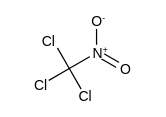
\includegraphics{smile-e94c93ea4e83a68999f255ede57b37121cf107e0}\\
(4)Freon - 12\\
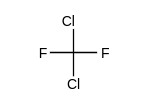
\includegraphics{smile-7127f10734ebf7ea0d8ef90481e34e7724c60ee7}\\
32. Incorrect statement for the use of indicators in acid-base titration is :\\
(1) Methyl orange may be used for a weak acid vs weak base titration.\\
(2) Methyl orange is a suitable indicator for a strong acid vs weak base titration\\
(3) Phenolphthalein is a suitable indicator for a weak acid vs strong base titration\\
(4) Phenolphthalein may be used for a strong acid vs strong base titration.\\
Official Ans. by NTA (1)\\
Allen Ans. (1)\\
Sol.

\begin{center}
\begin{tabular}{|l|l|}
\hline
Indicator & pH range \\
\hline
Methyl orange & \(3.2-4.5\) \\
\hline
Phenolpthalein & \(8.3-10.5\) \\
\hline
\end{tabular}
\end{center}

Methyl orange may be used for a strong acid vs strong base and strong acid vs weak base titration. Phenolpthalein may be used for a strong acid vs strong base and weak acid vs strong base titration.\\
33. Which of the following compounds are not used as disinfectants?

\section*{TEST PAPER WITH SOLUTION}
(A) Chloroxylenol\\
(B) Bithional\\
(C) Veronal\\
(D) Prontosil\\
(E) Terpineol

Choose the correct answer from the options given below:\\
(1) A, B, E\\
(2) A, B\\
(3) B, D, E\\
(4) C, D

Official Ans. by NTA (4)\\
Allen Ans. (1)\\
Sol. Veronal is neurological medicine, Prontosil is antibiotic, rest all are disinfectants.\\
34. A hydrocarbon ' X ' with formula \(\mathrm{C}_{6} \mathrm{H}_{8}\) uses two moles of \(\mathrm{H}_{2}\) on catalytic hydrogenation of its one mole. On ozonolysis, ' \(X\) ' yields two moles of methane dicarbaldehyde. The hydrocarbon ' X ' is :\\
(1) hexa-1, 3, 5-triene\\
(2) 1-methylcyclopenta-1, 4-diene\\
(3) cyclohexa-1, 3-diene\\
(4) cyclohexa-1, 4-diene

Official Ans. by NTA (4)\\
Allen Ans. (4)\\
Sol.\\
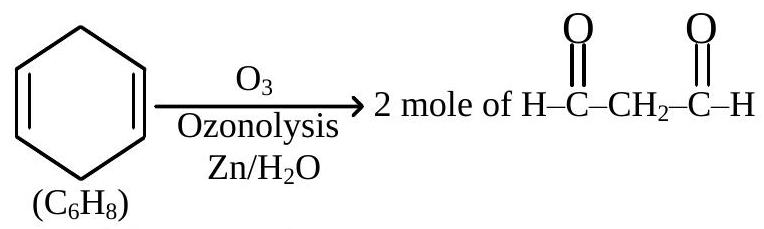
\includegraphics[max width=\textwidth, center]{2025_10_03_c0b598f36ce7f5fa9d3bg-1}\\
(Cyclohexa-1, 4-diene)\\
35. Cyclohexylamine when treated with nitrous acid yields (P). On treating (P) with PCC results in (Q). When (Q) is heated with dil. NaOH we get (R) The final product \((\mathrm{R})\) is :

(1)\\
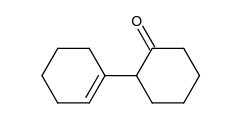
\includegraphics{smile-7f9d54f49efe534a57df8fda498a09783f199854}

(2)\\
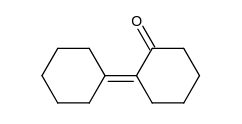
\includegraphics{smile-e8a4fbf8b2d0ea4f910f3ef7d3eec6fbd03027cb}

(3)\\
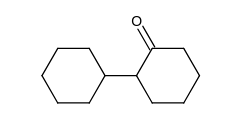
\includegraphics{smile-15a52ad396d7e5afe6a380e5b6352a7b870ed452}

(4)\\
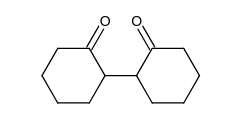
\includegraphics{smile-9f4b3aa718ab69379c7290c1ca921885c6d07c61}

Official Ans. by NTA (2)\\
Allen Ans. (2)\\
Sol.\\
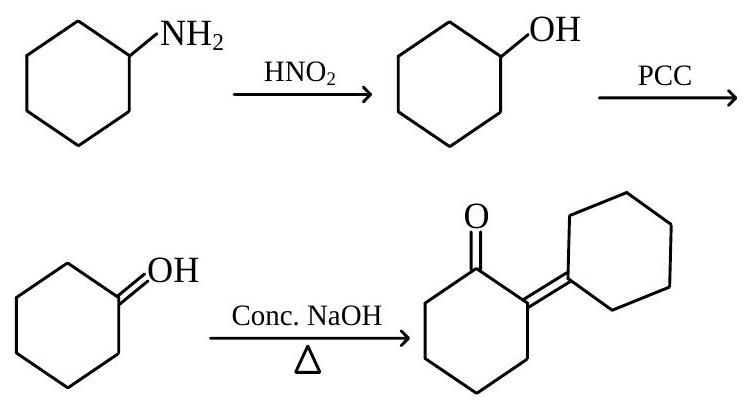
\includegraphics[max width=\textwidth, center]{2025_10_03_c0b598f36ce7f5fa9d3bg-2}\\
36. Given below are two statements:

Statement I: Upon heating a borax bead dipped in cupric sulphate in a luminous flame, the colour of the bead becomes green.\\
Statement II : The green colour observed is due to the formation of copper(I) metaborate.\\
In the light of the above statements, choose the most appropriate answer from the options given below :\\
(1) Both Statement I and Statement II are true\\
(2) Statement I is true but Statement II is false\\
(3) Both Statement I and Statement II are false\\
(4) Statement I is false but Statement II is true

Official Ans. by NTA (3)\\
Allen Ans. (3)\\
Sol. (Borax Bead Test)\\
On treatment with metal salt, boric anhydride forms metaborate of the metal which gives different colours in oxidising and reducing flame. For example, in the case of copper sulphate, following reactions occur.

\[
\begin{array}{r}
\mathrm{CuSO}_{4}+\mathrm{B}_{2} \mathrm{O}_{3} \xrightarrow[\text { (Oxidising) }]{\text { Non -luminous flame }} \\
\\
\text { Cupric metaborate } \\
\text { blue-green }
\end{array}
\]

Two reactions may take place in reducing flame (Luminous flame)\\
(i) The blue-green \(\mathrm{Cu}\left(\mathrm{BO}_{2}\right)_{2}\) is reduced to colourless cuprous metaborate as :

\[
\begin{aligned}
& 2 \mathrm{Cu}\left(\mathrm{BO}_{2}\right)_{2}+2 \mathrm{NaBO}_{2}+\mathrm{C} \xrightarrow[\text { flame }]{\text { Luminous }} \\
& 2 \mathrm{CuBO}_{2}+\mathrm{Na}_{2} \mathrm{~B}_{4} \mathrm{O}_{7}+\mathrm{CO}
\end{aligned}
\]

(ii) Cupric metaborate may be reduced to metallic copper and bead appears red opaque.

\[
\begin{aligned}
& 2 \mathrm{Cu}\left(\mathrm{BO}_{2}\right)_{2}+4 \mathrm{NaBO}_{2}+2 \mathrm{C} \xrightarrow[\text { flame }]{\text { Luminous }} \\
& 2 \mathrm{Cu}+2 \mathrm{Na}_{2} \mathrm{~B}_{4} \mathrm{O}_{7}+2 \mathrm{CO}
\end{aligned}
\]

\begin{enumerate}
  \setcounter{enumi}{36}
  \item Evaluate the following statements for their correctness.\\
(A) The elevation in boiling point temperature of water will be same for 0.1 M NaCl and 0.1 M urea.\\
(B) Azeotropic mixtures boil without change in their composition\\
(C) Osmosis always takes place from hypertonic to hypotonic solution\\
(D) The density of \(32 \% \mathrm{H}_{2} \mathrm{SO}_{4}\) solution having molarity 4.09 M is approximately \(1.26 \mathrm{~g} \mathrm{~mL}^{-1}\)\\
(E) A negatively charged sol is obtained when KI solution is added to silver nitrate solution.
\end{enumerate}

Choose the correct answer from the options given below :\\
(1) B, D, and E only\\
(2) A, B, and D only\\
(3) A and C only\\
(4) B and D only

Official Ans. by NTA (4)\\
Allen Ans. (4)\\
Sol. (A) \(\Delta \mathrm{T}_{\mathrm{b}} \propto \mathrm{i} \times \mathrm{c}\)\\
(B) Azeotropic mixtures have same composition in both liquid and vapour phase.\\
(C) Osmosis always takes place from hypotonic to hypertonic solution.\\
(D) \(\mathrm{M}=\frac{30 \times 10 \times 1.26}{98} \approx 4.09 \mathrm{M}\)\\
(E) When KI solutions is added to \(\mathrm{AgNO}_{3}\) solution, positively charged solution results due to adsorption of \(\mathrm{Ag}^{+}\)ions from dispersion medium

\[
\mathrm{AgI} / \mathrm{Ag}^{+}
\]

\section*{Positively charged}
\begin{enumerate}
  \setcounter{enumi}{37}
  \item Compound \(\mathrm{A}, \mathrm{C}_{5} \mathrm{H}_{10} \mathrm{O}_{5}\), given a tetraacetate with \(\mathrm{Ac}_{2} \mathrm{O}\) and oxidation of A with \(\mathrm{Br}_{2}-\mathrm{H}_{2} \mathrm{O}\) gives an acid, \(\mathrm{C}_{5} \mathrm{H}_{10} \mathrm{O}_{6}\). Reduction of A with HI gives isopentane. The possible structure of A is :\\
(1)\\
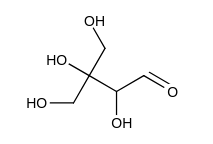
\includegraphics{smile-4f4aee5da4aa4ddc9f95428fae4f45a06bd3146c}\\
(2)\\
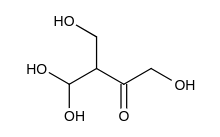
\includegraphics{smile-5196a79306e978d3197356dbe80dd168d700e558}\\
(3)\\
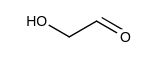
\includegraphics{smile-2a35f8ab75ae63cc03bb9a469fd941b1070fa573}\\
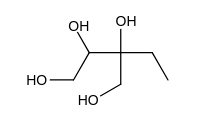
\includegraphics{smile-ac38716243519a71bdb9de8bb4c146df3030ca93}\\
(4)\\
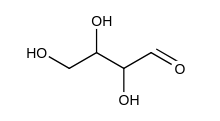
\includegraphics{smile-b9dc98270a42e05ae972d13450fbdd1bc340c62a}
\end{enumerate}

Official Ans. by NTA (1)\\
Allen Ans. (1)\\
Sol. (i) Formation of tetraacetete with \(\mathrm{Ac}_{2} \mathrm{O}\) means compound A has four -OH linkage.\\
Reduction of A with HI gives Isopentane i.e. molecule contains five carbon atom.\\
39. Arrange the following orbitals in decreasing order of energy?\\
(A) \(\mathrm{n}=3, \mathrm{l}=0, \mathrm{~m}=0\)\\
(B) \(\mathrm{n}=4, \mathrm{l}=0, \mathrm{~m}=0\)\\
(C) \(\mathrm{n}=3, \mathrm{l}=1, \mathrm{~m}=0\)\\
(D) \(\mathrm{n}=3,1=2, \mathrm{~m}=1\)

The correct option for the order is :\\
(1) \(\mathrm{B}>\mathrm{D}>\mathrm{C}>\mathrm{A}\)\\
(2) \(\mathrm{D}>\mathrm{B}>\mathrm{C}>\mathrm{A}\)\\
(3) A \(>\) C \(>\) B \(>\) D\\
(4) \(\mathrm{D}>\mathrm{B}>\mathrm{A}>\mathrm{C}\)

Official Ans. by NTA (2)\\
Allen Ans. (2)\\
Sol. (A) \(\mathrm{n}=3 ; 1=0 ; \mathrm{m}=0 ; 3 \mathrm{~s}\) orbital\\
(B) \(\mathrm{n}=4 ; \mathrm{l}=0 ; \mathrm{m}=0 ; 4 \mathrm{~s}\) orbital\\
(C) \(\mathrm{n}=3 ; 1=1 ; \mathrm{m}=0 ; 3 \mathrm{p}\) orbital\\
(D) \(\mathrm{n}=3 ; \mathrm{l}=2 ; \mathrm{m}=0 ; 3 \mathrm{~d}\) orbital

As per Hund's rule energy is given by ( \(\mathrm{n}+l\) ) value. If value of ( \(\mathrm{n}+l\) ) remains same then energy is given by n only.\\
40. The Lewis acid character of boron tri halides follows the order :\\
(1) \(\mathrm{BBr}_{3}>\mathrm{BI}_{3}>\mathrm{BCI}_{3}>\mathrm{BF}_{3}\)\\
(2) \(\mathrm{BCl}_{3}>\mathrm{BF}_{3}>\mathrm{BBr}_{3}>\mathrm{BI}_{3}\)\\
(3) \(\mathrm{BF}_{3}>\mathrm{BCl}_{3}>\mathrm{BBr}_{3}>\mathrm{BI}_{3}\)\\
(4) \(\mathrm{BI}_{3}>\mathrm{BBr}_{3}>\mathrm{BCl}_{3}>\mathrm{BF}_{3}\)

Official Ans. by NTA (4)\\
Allen Ans. (4)\\
Sol. Extent of back bonding, reduces down the group leading to more Lewis acidic strength\\
\(\mathrm{BF}_{3}>\mathrm{BCl}_{3}>\mathrm{BBr}_{3}>\mathrm{BI}_{3}\) (extent of back bonding) \((2 p-2 p)(2 p-3 p)(2 p-4 p)(2 p-5 p)\)\\
\(\mathrm{BF}_{3}<\mathrm{BCl}_{3}<\mathrm{BBr}_{3}<\mathrm{BI}_{3}\) (lewis acidic nature)\\
41. Match List-I with List-II

\begin{center}
\begin{tabular}{|c|l|c|l|}
\hline
\multicolumn{2}{|c|}{List-I} & \multicolumn{2}{c|}{List-II} \\
\hline
(A) & Physisorption & I & \begin{tabular}{l}
Single \\
layer adsorption \\
\end{tabular} \\
\hline
(B) & Chemisorption & II & \(20-40 \mathrm{~kJ} \mathrm{~mol}^{-1}\) \\
\hline
(C) & \(\mathrm{N}_{2}(\mathrm{~g})+3 \mathrm{H}_{2}(\mathrm{~g}) \xrightarrow{\mathrm{Fe}(\mathrm{s})} 2 \mathrm{NH}_{3}(\mathrm{~g})\) & III & Chromatography \\
\hline
(D) & \begin{tabular}{l}
Analytical Application \\
or Adsorption \\
\end{tabular} & IV & \begin{tabular}{l}
Heterogeneous \\
catalysis \\
\end{tabular} \\
\hline
\end{tabular}
\end{center}

Choose the correct answer from the options given below :\\
(1) A - II, B - III, C - I, D - IV\\
(2) \(\mathrm{A}-\mathrm{III}, \mathrm{B}-\mathrm{IV}, \mathrm{C}-\mathrm{I}\), \(\mathrm{D}-\mathrm{II}\)\\
(3) A - IV, B - II, C - III, D - I\\
(4) A - II, B - I, C - IV, D - III

Official Ans. by NTA (4)\\
Allen Ans. (4)\\
Sol. (A) Physisorption \(=20-40 \mathrm{~kJ} / \mathrm{mol}\) and Chemisorption \(=80-240 \mathrm{~kJ} / \mathrm{mol}\)\\
(B) Physisorption is multi-layered and chemisorption is unimolecular layered.\\
(C) In heterogeneous catalysis, medium and catalyst are in different phases.\\
(D) Chromatography uses adsorption to purify/separate mixtures.\\
42. Given below are two statements : one is labelled as Assertion (A) and the other is labelled as Reason (R)\\
Assertion (A) : The first ionization enthalpy of 3d series elements is more than that of group 2 metals\\
Reason (R) : In 3d series of elements successive filling of d-orbitals takes place.\\
In the light of the above statements, choose the correct answer from the options given below :\\
(1) Both (A) and (R) are true and (R) is the correct explanation of (A)\\
(2) Both (A) and (R) are true but (R) is not the correct explanation of (A)\\
(3) (A) is false but (R) is true\\
(4) (A) is true but ( \(\mathbf{R}\) ) is false

Official Ans. by NTA (1)\\
Allen Ans. (1)

Sol. From Sc to Mn ionization energy is less than that of Mg .

\section*{For 3d series :}
\begin{center}
\begin{tabular}{|c|c|c|c|c|c|}
\hline
 & Sc & Ti & V & Cr & Mn \\
\hline
\begin{tabular}{c}
IE \\
\((\mathrm{KJ} / \mathrm{mol})\) \\
\end{tabular} & 631 & 656 & 650 & 653 & 717 \\
\hline
 & Fe & Co & Ni & Cu & Zn \\
\hline
\begin{tabular}{c}
IE \\
\((\mathrm{KJ} / \mathrm{mol})\) \\
\end{tabular} & 762 & 758 & 736 & 745 & 906 \\
\hline
\end{tabular}
\end{center}

For \(2{ }^{\text {nd }}\) Group

\begin{center}
\begin{tabular}{|c|c|c|c|c|c|c|}
\hline
 & Be & Mg & Ca & Sr & Ba & Ra \\
\hline
\begin{tabular}{c}
IE \\
\((\mathrm{KJ} / \mathrm{mol})\) \\
\end{tabular} & 631 & 656 & 650 & 653 & 717 & 762 \\
\hline
\end{tabular}
\end{center}

\begin{enumerate}
  \setcounter{enumi}{42}
  \item The element playing significant role in neuromuscular function and interneuronal transmission is :\\
(1) Be\\
(2) Ca\\
(3) Li\\
(4) Mg
\end{enumerate}

Official Ans. by NTA (2)\\
Allen Ans. (2)\\
Sol. Calcium plays important role in neuromuscular function, interneuronal transmission, cell membrane etc.\\
44. Given below are two statements :

Statement I: \(\mathrm{H}_{2} \mathrm{O}_{2}\) is used in the synthesis of\\
Cephalosporin\\
Statement II: \(\mathrm{H}_{2} \mathrm{O}_{2}\) is used for the restoration of aerobic conditions to sewage wastes.\\
In the light of the above statements, choose the most appropriate answer from the options given below :\\
(1) Both Statement I and Statement II are correct\\
(2) Statement I is incorrect but Statement II is correct\\
(3) Statement I is correct but Statement II is incorrect\\
(4) Both Statement I and Statement II are incorrect

Official Ans. by NTA (1)\\
Allen Ans. (1)\\
Sol. It is used in the synthesis of hydroquinone, tartaric acid and certain food products and pharmaceuticals (cephalosporin) etc. Restoration of aerobic conditions to sewage wastes etc.\\
45. The normal rain water is slightly acidic and its pH value is 5.6 because of which one of the following?\\
(1) \(\mathrm{CO}_{2}+\mathrm{H}_{2} \mathrm{O} \rightarrow \mathrm{H}_{2} \mathrm{CO}_{3}\)\\
(2) \(4 \mathrm{NO}_{2}+\mathrm{O}_{2}+2 \mathrm{H}_{2} \mathrm{O} \rightarrow 4 \mathrm{HNO}_{3}\)\\
(3) \(2 \mathrm{SO}_{2}+\mathrm{O}_{2}+2 \mathrm{H}_{2} \mathrm{O} \rightarrow 2 \mathrm{H}_{2} \mathrm{SO}_{4}\)\\
(4) \(\mathrm{N}_{2} \mathrm{O}_{5}+\mathrm{H}_{2} \mathrm{O} \rightarrow 2 \mathrm{HNO}_{3}\)

Official Ans. by NTA (1)\\
Allen Ans. (1)\\
Sol. We are aware that normally rain water has a pH of 5.6 due to the presence of \(\mathrm{H}^{+}\)ions formed by the\\
reactions of rain water with carbon dioxide present in the atmosphere.\\
\(\mathrm{H}_{2} \mathrm{O}(\mathrm{l})+\mathrm{CO}_{2}(\mathrm{~g}) \leftrightharpoons \mathrm{H}_{2} \mathrm{CO}_{3}(\mathrm{aq})\)\\
\(\mathrm{H}_{2} \mathrm{CO}_{3}(\mathrm{aq}) \leftrightharpoons \mathrm{H}^{+}(\mathrm{aq})+\mathrm{HCO}_{3}^{-}(\mathrm{aq})\)\\
46. When a hydrocarbon A undergoes complete combustion it requires 11 equivalents of oxygen and produces 4 equivalents of water. What is the molecular formula of A ?\\
(1) \(\mathrm{C}_{9} \mathrm{H}_{8}\)\\
(2) \(\mathrm{C}_{11} \mathrm{H}_{4}\)\\
(3) \(\mathrm{C}_{5} \mathrm{H}_{8}\)\\
(4) \(\mathrm{C}_{11} \mathrm{H}_{8}\)

Official Ans. by NTA (1)\\
Allen Ans. (1)\\
Sol. \(\quad \mathrm{C}_{\mathrm{x}} \mathrm{H}_{\mathrm{y}}+\left(\mathrm{x}+\frac{\mathrm{y}}{4}\right) \mathrm{O}_{2} \rightarrow \mathrm{xCO}_{2}+\frac{\mathrm{y}}{2} \mathrm{H}_{2} \mathrm{O}\)\\
\(\frac{y}{2}=4 \therefore y=8\)\\
\(\mathrm{x}+\frac{8}{4}=11\)\\
\(\therefore \mathrm{x}=9\)\\
\(\therefore\) Hydrocarbon will be \(=\mathrm{C}_{9} \mathrm{H}_{8}\)\\
47. An organic compound \([\mathrm{A}]\left(\mathrm{C}_{4} \mathrm{H}_{11} \mathrm{~N}\right)\), shows optical activity and gives \(\mathrm{N}_{2}\) gas on treatment with \(\mathrm{HNO}_{2}\). The compound [A] reacts with \(\mathrm{PhSO}_{2} \mathrm{Cl}\) producing a compound which is soluble in KOH . The structure of A is:

(1)\\
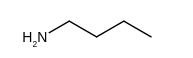
\includegraphics{smile-05a21dcdac94b68d9e739c2854228fe586e3bd96}

(2)\\
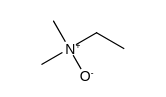
\includegraphics{smile-4889359965e5a0e808e98690e88972328bd10c82}

(3)\\
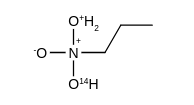
\includegraphics{smile-5bff8647005dab0beac93b9ce38e78993edf3437}

(4)\\
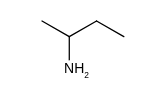
\includegraphics{smile-829fd2730c436045aea412c319d0d652e3f69568}

Official Ans. by NTA (4) Allen Ans. (4)

Sol. \(\mathrm{C}_{4} \mathrm{H}_{11} \mathrm{~N}\) releases \(\mathrm{N}_{2}\) with \(\mathrm{HNO}_{2}\) i.e. it is primary amine.\\
After reacting with Hinsberg reagent it forms a compound which is soluble in KOH , Hence, the amine is primary.\\
48. Which one of the following statements is incorrect?\\
(1) Boron and Indium can be purified by zone refining method.\\
(2) Van- Arkel method is used to purify tungsten.\\
(3) Cast iron is obtained by melting pig iron with scrap iron and coke using hot air blast.\\
(4) The malleable iron is prepared from cast iron by oxidising impurities in a reverberatory furnace.\\
Official Ans. by NTA (2)\\
Allen Ans. (2)\\
Sol. Van - Arkel process is used for purification of Ti, \(\mathrm{Zr}, \mathrm{Hf}\) and B .\\
49. Which of the following elements have half-filled f-orbitals in their ground state ?\\
(Given : atomic number\\
\(\mathrm{Sm}=62 ; \mathrm{Eu}=63 ; \mathrm{Tb}=65 ; \mathrm{Gd}=64, \mathrm{Pm}=61\) )\\
A. Sm\\
B. Eu\\
C. Tb\\
D. Gd\\
E. Pm

Choose the correct answer from the options given below:\\
(1) B and D only\\
(2) A and E only\\
(3) A and B only\\
(4) C and D only

Official Ans. by NTA (1)\\
Allen Ans. (1)\\
Sol. 1. \({ }_{62} \mathrm{Sm}: 4 \mathrm{f}^{6} 6 \mathrm{~s}^{2}\)\\
2. \({ }_{64} \mathrm{Gd}: 4 \mathrm{f}^{7} 5 \mathrm{~d}^{1} 6 \mathrm{~s}^{2}\)\\
3. \({ }_{63} \mathrm{Eu}: 4 \mathrm{f}^{7} 6 \mathrm{~s}^{2}\)\\
4. \({ }_{65} \mathrm{~Tb}: 4 \mathrm{f}^{9} 6 \mathrm{~s}^{2}\)\\
5. \({ }_{61} \mathrm{Pm}: 4 \mathrm{f}^{5} 6 \mathrm{~s}^{2}\)\\
50. In Dumas method for the estimation of \(\mathrm{N}_{2}\), the sample is heated with copper oxide and the gas evolved is passed over :\\
(1) Ni\\
(2) Copper gauze\\
(3) Pd\\
(4) Copper oxide

Official Ans. by NTA (2)\\
Allen Ans. (2)\\
Sol. Duma's method.\\
The nitrogen containing organic compound, when heated with CuO in a atmosphere of \(\mathrm{CO}_{2}\), yields free \(\mathrm{N}_{2}\) in addition to \(\mathrm{CO}_{2}\) and \(\mathrm{H}_{2} \mathrm{O}\).

\[
\begin{aligned}
& \mathrm{C}_{\mathrm{x}} \mathrm{H}_{\mathrm{y}} \mathrm{~N}_{\mathrm{z}}+\left(2 \mathrm{x}+\frac{\mathrm{y}}{2}\right) \mathrm{CuO} \rightarrow \\
& \quad \mathrm{x} \mathrm{CO}_{2}+\frac{\mathrm{y}}{2} \mathrm{H}_{2} \mathrm{O}+\frac{\mathrm{z}}{2} \mathrm{~N}_{2}+\left(2 \mathrm{x}+\frac{\mathrm{y}}{2}\right) \mathrm{Cu}
\end{aligned}
\]

Traces of nitrogen oxides formed, if any, are reduced to nitrogen by passing the gaseous mixture over heated copper gauze.

\section*{SECTION-B}
\begin{enumerate}
  \setcounter{enumi}{50}
  \item If the CFSE of \(\left[\mathrm{Ti}\left(\mathrm{H}_{2} \mathrm{O}\right)_{6}\right]^{3+}\) is \(-96.0 \mathrm{~kJ} / \mathrm{mol}\), this complex will absorb maximum at wavelength \(\_\_\_\_\) nm. (nearest integer)
\end{enumerate}

Assume Planck's constant \((\mathrm{h})=6.4 \times 10^{-34}\) Js Speed of light \((\mathrm{c})=3.0 \times 10^{8} \mathrm{~m} / \mathrm{s}\) and Avogadro's constant \(\left(\mathrm{N}_{\mathrm{A}}\right)=6 \times 10^{23} / \mathrm{mol}\).\\
Official Ans. by NTA (480)\\
Allen Ans. (480)\\
Sol. \(\left(\mathrm{Ti}^{+3}\left(\mathrm{H}_{2} \mathrm{O}\right)_{6}\right)^{3+}\)\\
\(\mathrm{Ti}^{+3}: 3 \mathrm{~d}^{\prime}\)

\[
\begin{aligned}
\text { C.F.S.E. } & =-0.4 \times \Delta_{0} \\
& =-\frac{96 \times 10^{3}}{\mathrm{~N}_{0}} \mathrm{~J}
\end{aligned}
\]

\[
\begin{aligned}
\Delta_{0} & =\frac{96 \times 10^{3}}{0.4 \times 6 \times 10^{23}} \\
\Rightarrow \quad \frac{\mathrm{hc}}{\lambda} & =\frac{96 \times 10^{3}}{0.4 \times 6 \times 10^{23}} \\
\lambda & =\frac{0.4 \times 6 \times 10^{23} \times 6.4 \times 10^{-34} \times 3 \times 10^{8}}{96 \times 10^{3}} \\
& =0.48 \times 10^{-6} \mathrm{~m} \\
& =480 \times 10^{-9} \mathrm{~m} \\
& =480 \mathrm{~nm}
\end{aligned}
\]

\begin{enumerate}
  \setcounter{enumi}{51}
  \item Amongst the following, the number of species having the linear shape is \(\_\_\_\_\) .\\
\(\mathrm{XeF}_{2}, \mathrm{I}_{3}^{+}, \mathrm{C}_{3} \mathrm{O}_{2}, \mathrm{I}_{3}^{-}, \mathrm{CO}_{2}, \mathrm{SO}_{2}, \mathrm{BeCl}\) and \(\mathrm{BCl}_{2}^{\Theta}\)\\
Official Ans. by NTA (5)\\
Allen Ans. (5)\\
Sol.\\
(i)\\
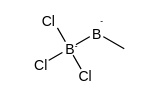
\includegraphics{smile-f6bc4d4734a7d0c217379eb6311a2468dcb157f0}\\
(ii) \(\mathrm{Cl}-\mathrm{Be}-\mathrm{Cl}\)
\end{enumerate}

\begin{figure}[h]
\begin{center}
\captionsetup{labelformat=empty}
\caption{(iii) (\textbackslash mathrm\{I}\_\{3\}\^{}\{-\})\}\\
  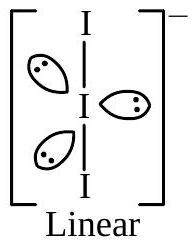
\includegraphics[width=\textwidth]{2025_10_03_c0b598f36ce7f5fa9d3bg-6(3)}
\end{center}
\end{figure}

\begin{figure}[h]
\begin{center}
\captionsetup{labelformat=empty}
\caption{(iv)}
  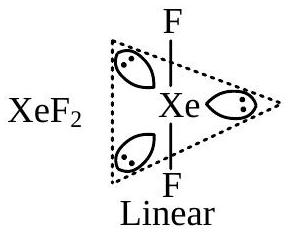
\includegraphics[width=\textwidth]{2025_10_03_c0b598f36ce7f5fa9d3bg-6(1)}
\end{center}
\end{figure}

\begin{figure}[h]
\begin{center}
\captionsetup{labelformat=empty}
\caption{(v)}
  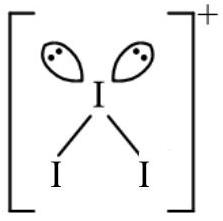
\includegraphics[width=\textwidth]{2025_10_03_c0b598f36ce7f5fa9d3bg-6(2)}
\end{center}
\end{figure}

V - Shape\\
(vi) \(\begin{gathered}\mathrm{CO}_{2} \quad \mathrm{O}=\mathrm{C}=\mathrm{O} \\ \text { Linear }\end{gathered}\)\\
(vii \(\mathrm{C}_{3} \mathrm{O}_{2}(\mathrm{O}=\mathrm{C}=\mathrm{C}=\mathrm{C}=\mathrm{O})\)\\
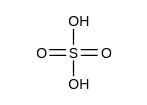
\includegraphics{smile-a45fda767311f6db8f45fdc0289e28045083d344}\\
53. The resistivity of a 0.8 M solution of an electrolyte is \(5 \times 10^{-3} \Omega \mathrm{~cm}\). Its molar conductivity is\\
\(\_\_\_\_\) \(\times 10^{4} \Omega^{-1} \mathrm{~cm}^{2} \mathrm{~mol}^{-1}\). (Nearest integer)

Official Ans. by NTA (25)\\
Allen Ans. (25)\\
Sol. \(\Lambda_{\mathrm{m}}=\frac{\kappa \times 1000}{\mathrm{M}}\)\\
\(\Lambda_{\mathrm{m}}=\frac{1}{\rho} \times \frac{1000}{\mathrm{M}}\)

\[
\frac{1}{5 \times 10^{-3}} \times \frac{1000}{0.8}
\]

Ans. \(25 \times 10^{4} \Omega^{-1} \mathrm{~cm}^{-2} \mathrm{~mol}^{-1}\)\\
54. At 298 K , the solubility of silver chloride in water is \(1.434 \times 10^{-3} \mathrm{~g} \mathrm{~L}^{-1}\). The value of \(-\log \mathrm{K}_{\text {sp }}\) for silver chloride is \(\_\_\_\_\) .\\
(Given mass of Ag is \(107.9 \mathrm{~g} \mathrm{~mol}^{-1}\) and mass of Cl is \(35.5 \mathrm{~g} \mathrm{~mol}^{-1}\) )\\
Official Ans. by NTA (10)\\
Allen Ans. (10)\\
Sol. \(\quad \operatorname{AgCl}(\mathrm{s}) \rightarrow \mathrm{Ag}^{+}(\mathrm{aq})+.\mathrm{Cl}^{-}(\mathrm{aq}\).\\
S S\\
\(\mathrm{K}_{\text {sp }}=\mathrm{S}^{2}=\left(\frac{1.43}{143.4} \times 10^{-3}\right)^{2}=10^{-10}\)\\
\(-\log \mathrm{K}_{\mathrm{sp}}=10\)\\
55. A sample of a metal oxide has formula \(\mathrm{M}_{0.83} \mathrm{O}_{1.00}\). The metal M can exist in two oxidation states +2 and +3 . In the sample of \(\mathrm{M}_{0.83} \mathrm{O}_{1.00}\), the percentage of metal ions existing in +2 oxidation state is \(\_\_\_\_\) \% (nearest integer)\\
Official Ans. by NTA (59)\\
Allen Ans. (59)\\
Sol.\\
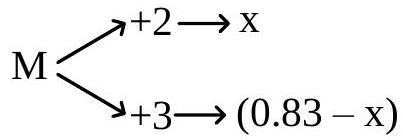
\includegraphics[max width=\textwidth, center]{2025_10_03_c0b598f36ce7f5fa9d3bg-6}\\
\(2 x+3(0.83-x)=2\)\\
\(x=0.49\)\\
\(\% M^{2+}=\frac{0.49}{0.83} \times 100\)\\
= 59\%\\
56. Assume carbon burns according to following equation :\\
\(2 \mathrm{C}_{(\mathrm{s})}+\mathrm{O}_{2(\mathrm{~g})} \rightarrow 2 \mathrm{CO}(\mathrm{g})\)\\
When 12 g carbon is burnt in 48 g of oxygen, the volume of carbon monoxide produced is \(\_\_\_\_\) \(\times 10^{-1} \mathrm{~L}\) at STP [nearest integer]\\[0pt]
[Given : Assume CO as ideal gas, Mass of C is \(12 \mathrm{~g} \mathrm{~mol}^{-1}\), Mass of O is \(16 \mathrm{~g} \mathrm{~mol}^{-1}\) and molar volume of an ideal gas at STP is \(22.7 \mathrm{~L} \mathrm{~mol}^{-1}\) ]\\
Official Ans. by NTA (227)\\
Allen Ans. (227)\\
Sol. \(\quad 2 \mathrm{C}(\mathrm{s})+\mathrm{O}_{2}(\mathrm{~g}) \rightarrow 2 \mathrm{CO}(\mathrm{g})\)\\
\(1 \mathrm{~mol} \quad 1.5 \mathrm{~mol}\)\\
Limiting reagent is carbon. One mole carbon produces one mole CO . Hence, volume at STP is \(227 \times 10^{-1}\) litre\\
57. The number of alkali metal(s), from \(\mathrm{Li}, \mathrm{K}, \mathrm{Cs}, \mathrm{Rb}\) having ionization enthalpy greater than \(400 \mathrm{~kJ} \mathrm{~mol}^{-1}\) and forming stable super oxide is \(\_\_\_\_\) .\\
Official Ans. by NTA (2)\\
Allen Ans. (2)\\
Sol. \(\mathrm{K}, \mathrm{Rb}\) and Cs form stable super oxides but Cs has ionisation enthalpy less than 400 kJ .\\
58. Enthalpies of formation of \(\mathrm{CCl}_{4}(\mathrm{~g}), \mathrm{H}_{2} \mathrm{O}(\mathrm{g}), \mathrm{CO}_{2}(\mathrm{~g})\) and\\
\(\mathrm{HCl}(\mathrm{g})\) are \(-105,-242,-394\) and \(-92 \mathrm{~kJ} \mathrm{~mol}^{-1}\) respectively. The magnitude of enthalpy of the reaction given below is \(\_\_\_\_\) \(\mathrm{kJ} \mathrm{mol}^{-1}\)\\
(nearest integer)\\
\(\mathrm{CCl}_{4}(\mathrm{~g})+2 \mathrm{H}_{2} \mathrm{O}(\mathrm{g}) \rightarrow \mathrm{CO}_{2}(\mathrm{~g})+4 \mathrm{HCl}(\mathrm{g})\)\\
Official Ans. by NTA (173)\\
Allen Ans. (173)\\
Sol. \(\Delta_{\mathrm{r}} \mathrm{H}=\sum \mathrm{H}_{\mathrm{p}}-\sum \mathrm{H}_{\mathrm{R}}\)\\
\(=(-394+4 \times-92)-(-105+(2 \times-242))\)\\
\(=-173 \mathrm{~kJ} / \mathrm{mol}\)\\
59. The number of molecules which gives haloform test among the following molecules is \(\_\_\_\_\) .\\
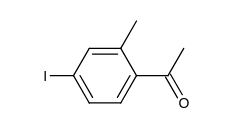
\includegraphics{smile-58703be8abbae173221b8b8745e0f69c6319073d}\\
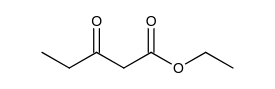
\includegraphics{smile-fd966806f2c2bca229d828ccaa1d4dd1106bb8e9}\\
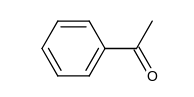
\includegraphics{smile-5ed6870f5dd90f0938579beeb78f4c499ffef574}\\
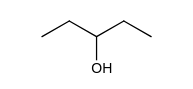
\includegraphics{smile-c9aedab809afea98e889cf4e57b9cb550a0c1fe3}\\
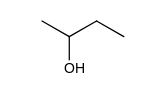
\includegraphics{smile-7bfb0cbbe5e76593e4012189eb218c067306e74e}\\
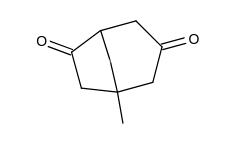
\includegraphics{smile-474455481d923ea27e7212ed52f215c556b05978}

Official Ans. by NTA (3)\\
Allen Ans. (3)\\
Sol.\\
Molecules having\\
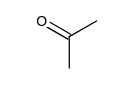
\includegraphics{smile-0f5da6af577e060e1f42c3d272bc0879d9bcae72}\\
and\\
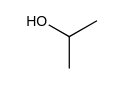
\includegraphics{smile-006160811eb757853c70df66f83c950b4498a67f}\\
gives positive haloform test.\\
60. The rate constant for a first order reaction is \(20 \mathrm{~min}^{-1}\). The time required for the initial concentration of the reactant to reduce to its \(\frac{1}{32}\) level is \(\_\_\_\_\) \(\times 10^{-2} \mathrm{~min}\). (Nearest integer)\\
(Given :

\[
\begin{aligned}
& \ln 10=2.303 \\
& \log 2=0.3010)
\end{aligned}
\]

Official Ans. by NTA (17)\\
Allen Ans. (17)\\
Sol.

\[
\begin{aligned}
\mathrm{C}=\frac{\mathrm{C}_{\mathrm{o}}}{2^{\mathrm{n}}} & =\frac{\mathrm{C}_{\mathrm{o}}}{32} \\
\mathrm{n} & =5 \\
\mathrm{t} & =5 \mathrm{t}_{1 / 2} \\
& =\frac{5 \times 0.693}{20}=\frac{0.693}{4} \\
& =0.17325 \mathrm{~min}=17.325 \times 10^{-2} \mathrm{~min}
\end{aligned}
\]


\end{document}